\documentclass{article}
\usepackage[yyyymmdd]{datetime}
\usepackage[nottoc]{tocbibind}
\usepackage{pgfplots}
\pgfplotsset{compat=1.18}
\usepackage{url}
\usepackage{array}
\usepackage{float}
\usepackage[inline,shortlabels]{enumitem}
\usepackage{hhline}
\usepackage{multirow}
\usepackage{geometry}
\usepackage[dvipsnames]{xcolor}
\usepackage{colortbl}
\usepackage[framemethod=TikZ]{mdframed}
\usepackage{amsfonts}
\usepackage{amsmath}
\usepackage{tikz}
\usepackage{amsthm}
\newtheoremstyle{problemstyle}{3pt}{3pt}{\normalfont}{}{\bfseries}{\normalfont\bfseries:}{.5em}{}
\theoremstyle{problemstyle}
\newmdtheoremenv[
  linewidth=1pt,
  linecolor=RoyalBlue,
  backgroundcolor=RoyalBlue!10,
  roundcorner=5pt,
  innertopmargin=6pt,
  innerbottommargin=6pt,
  innerleftmargin=6pt,
  innerrightmargin=6pt,
  nobreak=true
]{problem}{Problem}

% Example
\newmdtheoremenv[
  linewidth=1pt,
  linecolor=ForestGreen,
  backgroundcolor=ForestGreen!10,
  roundcorner=5pt,
  nobreak=true
]{example}{Example}

% Theorem
\newmdtheoremenv[
  linewidth=1pt,
  linecolor=BrickRed,
  backgroundcolor=BrickRed!10,
  roundcorner=5pt,
  nobreak=true
]{theorem}{Theorem}

% Remark
\newmdtheoremenv[
  linewidth=1pt,
  linecolor=Goldenrod,
  backgroundcolor=Goldenrod!10,
  roundcorner=5pt,
  nobreak=true
]{remark}{Remark}

% Solution
\newenvironment{solution}{%
  \begin{mdframed}[linewidth=0.8pt,linecolor=Gray,backgroundcolor=Gray!5,roundcorner=5pt]%
  \noindent\textbf{Solution.}%
}{%
\hfill $ \diamond $ 
  \end{mdframed}%
}

\usepackage{listings}

\lstset{breaklines=true}
\definecolor{vscode-blue}{RGB}{64, 116, 160}   % Keywords
\definecolor{vscode-green}{RGB}{95, 203, 114}   % Strings
\definecolor{vscode-gray}{RGB}{128, 128, 128}   % Comments
\definecolor{vscode-orange}{RGB}{206, 145, 120} % Numbers/Constants
\definecolor{vscode-purple}{RGB}{204, 124, 255} % Functions/Types
\definecolor{vscode-cyan}{RGB}{155, 199, 217}   % Preprocessor

\lstdefinestyle{visual-studio}{
    language=C,
    backgroundcolor=\color{Gray!5},
    commentstyle=\color{vscode-gray}\ttfamily,
    keywordstyle=\color{vscode-blue}\ttfamily,
    stringstyle=\color{vscode-green}\ttfamily,
    numberstyle=\color{vscode-orange}\ttfamily,
    identifierstyle=\color{black}\ttfamily,
    breaklines=true,
    showstringspaces=false,
    tabsize=4,
    % Additional settings for more Visual Studio feel
    emph=[1]{void, int, double, float, char, bool, short, long, signed, unsigned, class, struct, enum, union, typedef, template}, % Common types
    emphstyle=[1]\color{vscode-purple},
    emph=[2]{printf, scanf, cin, cout, return, new, delete, if, else, while, do, for, switch, case, default, break, continue, goto, throw, try, catch, const, static, extern, volatile, register, restrict, inline, explicit, virtual, friend, namespace, using, private, protected, public, operator}, % Standard keywords
    emphstyle=[2]\color{vscode-blue},
            keywordstyle=[2]\color{vscode-cyan}\ttfamily\bfseries,
    morekeywords={\#include, \#define, \#ifdef, \#ifndef, \#endif, \#pragma},
    basicstyle=\small
}

% Make header with name and date etc.
\usepackage{fancyhdr}
\lhead{Pedro D. Llerenas\\M\'etodos Num\'ericos I}
\rhead{\today\\Tarea II}
\thispagestyle{fancy}

\usepackage[utf8]{inputenc}
\setlength{\parindent}{0pt} % Don't indent new paragraphs
\setlength{\headheight}{24pt} 

\newcommand{\Z}{\mathbb Z}
\newcommand{\Q}{\mathbb Q}
\newcommand{\R}{\mathbb R}
\newcommand{\C}{\mathbb C}
\newcommand{\N}{\mathbb N}


\begin{document}

\section*{M\'etodos iterativos para ecuaciones no lineales}\label{chap:m_etodos_iterativos_para_ecuaciones_no_lineales} % (fold)

% chapter M\'etodos iterativos para ecuaciones no lineales (end)
\begin{problem}
Escribe un programa para calcular la constante matem\'atica $ e $, considerando la definici\'on
\[
	e = \lim_{n\to\infty} \left(1+\frac{1}{n}\right)^{n},
\]
es decir, calcula $ (1+1/n)^n $ para $ n = 10^k $, $ k = 1, 2,\dots, 20. $ Determina el error relativo y absoluto de las aproximaciones compar\'andolas con $ \exp(1) $. \textbf{(1 punto)}
\end{problem}
\begin{solution}
	\lstinputlisting[style=visual-studio, caption=Calcula el n-\'esimo t\'ermino del l\'imite de e, language=C, breaklines=true]{./Code/p1.c}

	Este nos genera la list
	\begin{align*}
		e_{10^{1}}  & = 2.593742460100002 \\
		e_{10^{2}}  & = 2.704813829421528 \\
		e_{10^{3}}  & = 2.716923932235594 \\
		e_{10^{4}}  & = 2.718145926824926 \\
		e_{10^{5}}  & = 2.718268237192297 \\
		e_{10^{6}}  & = 2.718280469095753 \\
		e_{10^{7}}  & = 2.718281694132082 \\
		e_{10^{8}}  & = 2.718281798347358 \\
		e_{10^{9}}  & = 2.718282052011560 \\
		e_{10^{10}} & = 2.718282053234788 \\
		e_{10^{11}} & = 2.718282053357110 \\
		e_{10^{12}} & = 2.718523496037238 \\
		e_{10^{13}} & = 2.716110034086901 \\
		e_{10^{14}} & = 2.716110034087023 \\
		e_{10^{15}} & = 3.035035206549262 \\
		e_{10^{16}} & = 1.000000000000000 \\
		e_{10^{17}} & = 1.000000000000000 \\
		e_{10^{18}} & = 1.000000000000000 \\
		e_{10^{19}} & = 1.000000000000000 \\
		e_{10^{20}} & = 1.000000000000000
	\end{align*}
	Notemos que en el t\'ermino 15, la computadora deja de producir un valor prudente. Esto se debe a que un doble tiene precision de 15 digitos. Para este punto, $1/10^{15}$ tiene el decimal en el \'ultimo punto de precisi\'on. Entonces, al elevar a este mismo t\'ermino, quedamos con algo que ser\'a impreciso. Para el t\'ermino 16, $1/10^{16}$ ya es redondeado a 0 por el sistema. Entonces, solamente nos queda $ 1^{10^k} = 1 $.

	Ahora, observemos que los errores son los siguientes:
	\begin{figure}[H]
		\begin{center}
			\begin{tabular}{r|r}
        \hline
				Absolute Error & Relative Error \\\hline
				1.245394e-01   & 4.801532e-02   \\
				1.346800e-02   & 4.979270e-03   \\
				1.357896e-03   & 4.997918e-04   \\
				1.359016e-04   & 4.999792e-05   \\
				1.359127e-05   & 4.999973e-06   \\
				1.359363e-06   & 5.000821e-07   \\
				1.343270e-07   & 4.941613e-08   \\
				3.011169e-08   & 1.107747e-08   \\
				2.235525e-07   & 8.224037e-08   \\
				2.247757e-07   & 8.269037e-08   \\
				2.248981e-07   & 8.273537e-08   \\
				2.416676e-04   & 8.889663e-05   \\
				2.171794e-03   & 7.995973e-04   \\
				2.171794e-03   & 7.995973e-04   \\
				3.167534e-01   & 1.043656e-01   \\
				1.718282e+00   & 1.718282e+00   \\
				1.718282e+00   & 1.718282e+00   \\
				1.718282e+00   & 1.718282e+00   \\
				1.718282e+00   & 1.718282e+00   \\
				1.718282e+00   & 1.718282e+00 
			\end{tabular}
		\end{center}
		\caption{Tabla de errores absolutos y relativos de aproximaciones a $e$.}\label{fig:errors}
	\end{figure}

\end{solution}

\begin{problem}
La ecuaci\'on $ x^3+x = 6 $ tiene una ra\'iz en el intervalo $ [1.55, 1.75] $, ¿cu\'antas iteracions se necesitan para obtener una aproximaci\'on de la raiz con error menor a 0.0001 con el m\'etodo de bisecci\'on? Verifica con el m\'etodo de bisecci\'on tu predicci\'on de la ra\'iz. \textbf{(2 puntos)}
\end{problem}
\begin{solution}
	Obtenemos la ra\'iz $ 1.634277 $ despu\'es de 11 iteraciones. A continuaci\'on, el programa utilizado.
	\lstinputlisting[style=visual-studio, caption=Programa que encuentra la raiz de un polinomio en un intervalo, language=C]{./Code/p2.c}
\end{solution}

\begin{problem}
Hallar una ra\'iz de $ f(x) = x^4 + 3x^2 - 2 $ por medio de las siguientes 4 formulaciones de punto fijo utilizando $ p_0 = 1 $:
\begin{center}
	\begin{enumerate*}[label=\alph*),itemjoin=\qquad]

		\item $\displaystyle x = \sqrt{\frac{2-x^4}{3}} $,
		\item $\displaystyle x = (2-3x^2)^{\frac{1}{4}}$,
		\item $\displaystyle x = \frac{2-x^4}{3x} $,
		\item $\displaystyle x = \left(\frac{2-3x^2}{x}\right)^{\frac{1}{3}}$
	\end{enumerate*}
\end{center}

\begin{enumerate}
	\item Las ra\'ices de $ f(x) $ deben de coincidir con las ra\'ices de $ x-g(x) $. Grafica $ f(x) $ y $ x-g(x) $. Comenta lo observado. \textbf{(1 punto)}

	\item Crea una tabla comparativa para comparar el resultado de las ra\'ices de $f(x) $ con la ra\'iz alcanzada con cada una de las formulaciones. Usa m\'aximo 20 iteraciones y tol = 0.0001. Explica lo sucedido. \textbf{(2 puntos)}
\end{enumerate}
\end{problem}
\begin{solution}
	\begin{figure}[H]
		\begin{center}
			\begin{minipage}{0.4\textwidth}
				\begin{tikzpicture}[scale=0.7]
					\begin{axis}[
							title={$f(x), x - g_1(x)$},
							xlabel={$x$},
							ylabel={$y$},
							axis lines=center,
							xmin=-2, xmax=2,
							ymin=-3, ymax=3,
							domain=-3:3,
							samples=100,
							legend pos=north east
						]
						\addplot[blue, thick] {x - sqrt((2-x*x*x*x)/3)};
						\addplot[red,thick] {x*x*x*x + 3*x*x - 2};
						\addlegendentry{$x - \sqrt{\frac{2-x^4}{3}}$} % This adds the label to the legend
						\addlegendentry{$x^4 + 3x^2 - 2$} % This adds the label to the legend
					\end{axis}
				\end{tikzpicture}
			\end{minipage}
			\begin{minipage}{0.4\textwidth}
				\begin{tikzpicture}[scale=0.7]
					\begin{axis}[
							title={$f(x), x - g_2(x)$},
							xlabel={$x$},
							ylabel={$y$},
							axis lines=center,
							xmin=-2, xmax=2,
							ymin=-3, ymax=3,
							domain=-3:3,
							samples=1000,
							legend pos=north east
						]
						\addplot[blue, thick] {x - (2-3*x*x)^(0.25)};
						\addplot[red,thick] {x*x*x*x + 3*x*x - 2};
						\addlegendentry{$ x - (2-3x^2)^{1/4}$} % This adds the label to the legend
						\addlegendentry{$x^4 + 3x^2 - 2$} % This adds the label to the legend
					\end{axis}
				\end{tikzpicture}
			\end{minipage}
		\end{center}
		\caption{Gr\'aficas de $ g_1 $ y $ g_2 $.}\label{fig:g1}
	\end{figure}

	\begin{figure}[H]
		\begin{center}
			\begin{minipage}{0.4\textwidth}
				\begin{tikzpicture}[scale=0.7]
					\begin{axis}[
							title={$f(x), x - g_3(x)$},
							xlabel={$x$},
							ylabel={$y$},
							axis lines=center,
							xmin=-2, xmax=2,
							ymin=-3, ymax=3,
							domain=-3:3,
							samples=1000,
							unbounded coords=jump,
							legend pos=north east
						]
						\addplot[blue, thick, domain=-2:-0.1] {x - (2-x^4)/(3*x)};
						\addplot[blue, thick, domain=0.1:2] {x - (2-x^4)/(3*x)};
						\addplot[red,thick] {x*x*x*x + 3*x*x - 2};
						\addlegendentry{$x - \sqrt{\frac{2-x^4}{3}}$} % This adds the label to the legend
						\addlegendentry{$x^4 + 3x^2 - 2$} % This adds the label to the legend
					\end{axis}
				\end{tikzpicture}
			\end{minipage}
			\begin{minipage}{0.4\textwidth}
				\begin{tikzpicture}[scale=0.7]
					\begin{axis}[
							title={$f(x), x - g_4(x)$},
							xlabel={$x$},
							ylabel={$y$},
							axis lines=center,
							xmin=-2, xmax=2,
							ymin=-3, ymax=3,
							domain=-3:3,
							samples=1000,
							unbounded coords=jump,
							legend pos=north east
						]
						\addplot[blue, thick, domain=-2:-0.1] {x - ((2-3*x^2)/x)^(1/3)};
						\addplot[blue, thick, domain=0.1:2] {x - ((2-3*x^2)/x)^(1/3)};
						\addplot[red,thick] {x*x*x*x + 3*x*x - 2};
						\addlegendentry{$ x - (\frac{2-3x^2}{x})^{1/3}$} % This adds the label to the legend
						\addlegendentry{} % This adds the label to the legend

						\addlegendentry{$x^4 + 3x^2 - 2$} % This adds the label to the legend
					\end{axis}
				\end{tikzpicture}
			\end{minipage}
		\end{center}
		\caption{Gr\'aficas de $g_3$ y $ g_4 $}\label{fig:g2}
	\end{figure}

	Observamos que en todos los casos, $ f(x) $ y $ x - g_i(x) $ tienen una ra\'iz en el mismo punto. Esto quiere decir que, efectivamente, encontrar un punto fijo de $ g_i $ nos proporciona una ra\'iz de $ f $.

	\lstinputlisting[style=visual-studio, caption=Programa que encuentra la raiz de un polinomio mediante la iteracion de punto fijo, language=C]{./Code/p3.c}
	El programa nos proporciona una archivo \texttt{p3.csv} con los siguientes valores:
	\begin{figure}[H]
		\begin{center}
			\begin{tabular}{c|c|c|c}
				$g_1(x)$ & $g_2(x)$ & $g_3(x)$           & $g_4(x)$  \\ \hline
				0.577350 & -nan     & 0.333333           & -1.000000 \\
				0.793492 & -nan     & 1.987654           & 1.000000  \\
				0.731110 & -nan     & -2.282184          & -1.000000 \\
				0.755929 & -nan     & 3.670032           & 1.000000  \\
				0.746876 & -nan     & -16.295738         & -1.000000 \\
				0.750296 & -nan     & 1442.409546        & 1.000000  \\
				0.749020 & -nan     & -1000332864.000000 & -1.000000 \\
				0.749498 & -nan     & 3.33e30            & 1.000000  \\
				0.749320 & -nan     & -inf               & -1.000000 \\
				0.749387 & -nan     & -nan               & 1.000000  \\
				0.749361 & -nan     & -nan               & -1.000000 \\
				0.749371 & -nan     & -nan               & 1.000000  \\
				0.749367 & -nan     & -nan               & -1.000000 \\
				0.749369 & -nan     & -nan               & 1.000000  \\
				0.749368 & -nan     & -nan               & -1.000000 \\
				0.749368 & -nan     & -nan               & 1.000000  \\
				0.749368 & -nan     & -nan               & -1.000000 \\
				0.749368 & -nan     & -nan               & 1.000000  \\
				0.749368 & -nan     & -nan               & -1.000000 \\
				0.749368 & -nan     & -nan               & 1.000000
			\end{tabular}
		\end{center}
		\caption{Tabla de itereciones de m\'etodo de punto fijo.}\label{fig:root_table}
	\end{figure}
	Notemos que solamente la funci\'on $ g_1 $ converge a un valor. $ g_2 $ falla por la elecci\'on del punto inicial, ya que $ g_2(1) $ no es un n\'umero real. $ g_3 $ diverge, ya que no se cumple que $ |g_3'(x)| < 1 $ para todo $ x\in (a,b)\subset [0,1] $, con $ a,b\in \R $ y $ a<b $. Finalmente, $ g_4 $ falla nuevamente por el punto inicial, ya que $ g_4(1) = -1 $ y $ g_4(-1) = 1 $. Entonces, este nunca converge a un valor.

\end{solution}

\begin{problem}
Utiliza el m\'etodo de bisecci\'on, m\'etodo de Newton, m\'etodo de la secante y m\'etodo de la falsa posici\'on para comparar los resultados de los siguientes problemas:
Encontrar $ \lambda $ con una presici\'on de $ 10^{-4} $ y $ N_{iter, max} = 100 $, para a ecuaci\'on de la poblaci\'on en t\'erminos de la tasa de natalidad $ \lambda $,
\[
	P(\lambda) = 1,000,000 e^{\lambda} + \frac{435,000}{\lambda}(e^{\lambda} - 1)
\]
para $ P(\lambda) = 1,564,000 $ individuos por a\~nos. Usa $ \lambda_0 = 0.01 $. (Sugerencia: graficar $ P(\lambda) - N $) \textbf{(4 puntos)}
\end{problem}

\begin{solution}
	\lstinputlisting[style=visual-studio, caption=Programa que encuentra la raiz de $P(\lambda)$, language=C]{./Code/p4.c}
	El programa nos proporciona 3 respuestas:\\
	\texttt{newton found root at 0.100989}\\
	\texttt{P(0.100989) = -11.865183}\\
	\texttt{secant found root at 0.096758}\\
	\texttt{P(0.096758) = -5666.057541}\\
	\texttt{False position's method failed after N = 100 iterations.}\\
	\texttt{root at 0.000000}\\
	\texttt{P(0.000000) = -nan}

	Entonces, el m\'etodo de Newton y de la secante lograron encontrar un valor $ \lambda $ tal que $ P(\lambda)$ se acerca a $1,564,000 $, mientras que el de falsa posici\'on fall\'o al no converger dentro de las 100 iteraciones.
\end{solution}
\end{document}
